\chapter{OSPF}

\section{Overview}

\subsection{Operation}

\begin{enumerate}
\item \textbf{Establish neighbor adjacencies:} An OSPF-enabled router sends Hello packets out all OSPF-enabled interfaces to determine if neighbors are present on those links.

\item \textbf{Building the Link-State Packets:} Each router builds a link-state packet (LSP) containing the state of \emph{each} directly connected link. 

\item \textbf{Flooding the LSP:} Routers flood their LSPs to all neighbors. To do this, whenever a router receives an LSP from a neighboring router, it immediately sends that LSP out all other interfaces, except the interface that received the LSP. This process creates a flooding effect of LSPs from all routers throughout the routing area.

\item \textbf{Build the Topology Table:} Routers build the topology table (LSDB) based on the received LSPs. 

\item \textbf{Execute the SPF Algorithm:} Routers use the SPF algorithm to create the SPF tree.

\item \textbf{Insert best path to routing table:} From the SPF tree, the best paths are inserted to the IP routing table. The route will remain the routing table unless there is another route with lower administrative distance (AD). Routing decisions are made based on the entries in the routing table, not LSDB.
\end{enumerate}
	
\subsection{OSPF network types}

OSPF defines five network types:

\begin{itemize}
	\item \textbf{Point-to-point} -- Two routers interconnected over a common link. No other routers are on the link. (Figure \ref{point-to-point})
	\item \textbf{Multiaccess} -- Multiple routers interconnected over a switch. (Figure \ref{multiaccess})
	\item \textbf{Nonbroadcast multiaccess (NBMA)} -- Multiple routers interconnected in a network that does not allow broadcasts, such as Frame Relay. (Figure \ref{NBMA})
	\item \textbf{Point-to-multipoint} -- Multiple routers interconnected in a hub-and-spoke topology over an NBMA network (Figure \ref{point-to-multipoin}).
	\item \textbf{Virtual links} -- Special OSPF network used to interconnect distant OSPF areas to the backbone area (Figure \ref{virtual-link}). In this scenario, area 51 cannot connect directly to area 0. A special OSPF area must be configured to connect area 51 to area 0. The R1 and R2 in area 1 must be configured as a virtual link.
\end{itemize}
	
\begin{figure}%
	\centering
	\subfigure[Point-to-point]{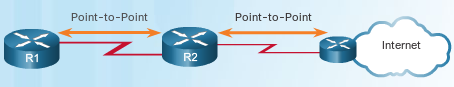
\includegraphics[width=0.4\textwidth]{point-to-point.png} \label{point-to-point}}
	\subfigure[Multiaccess]{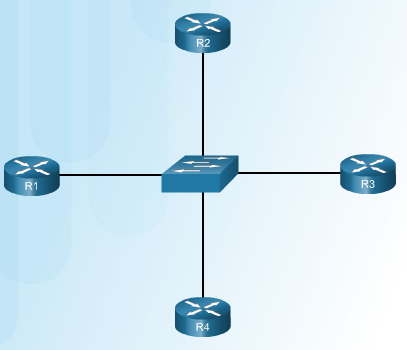
\includegraphics[width=0.4\textwidth]{multiaccess.png} \label{multiaccess}}
	\subfigure[Nonbroadcast multiaccess]{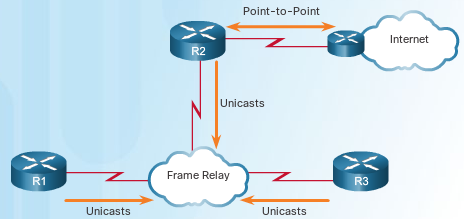
\includegraphics[width=0.4\textwidth]{pictures/NBMA.png} \label{NBMA}}
	\subfigure[Point-to-multipoint]{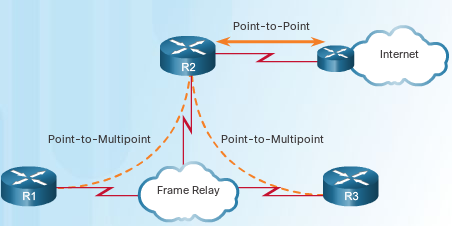
\includegraphics[width=0.4\textwidth]{pictures/point-to-multipoint.png} \label{point-to-multipoin}}
	\subfigure[Virtual link]{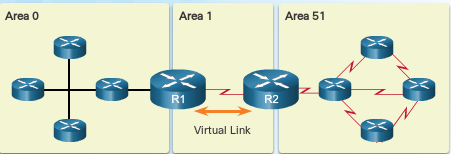
\includegraphics[width=0.4\textwidth]{pictures/virtual-link.png} \label{virtual-link}}
	\caption{OSPF network types}
	\label{network-types}
	\end{figure}
	
\subsection{OSPF cost}

OSPF uses \textbf{cost} as a metric, where lower cost indicates a better path. The cost of an interface is inversely proportional to the bandwidth of the interface:
\[ \text{cost}=\frac{\text{Reference bandwidth}}{\text{Interface bandwidth}} \]
The default reference bandwidth is 100 Mb/s, therefore the formula is:
\[ \text{cost}=\frac{10^8}{\text{Interface bandwidth in bps}} \]
Notice that any interfaces faster than 100 Mb/s share the same cost 1, because the OSPF cost value must be an integer. To avoid this, changing reference bandwidth to a higher value than 100 Mb/s is required. \\

\note Changing the reference bandwidth does not actually affect the physical bandwidth of the device; rather, it simply affects the calculation used to determine the metric.

\section{Protocol components}
The OSPF routing protocol has three main components:
\begin{itemize}
	\item Data structures
	\item Routing protocol messages
	\item Algorithm
	\end{itemize}
	
\subsection{Data structure}

Data structures are the tables or databases that OSPF builds in order to operate. OSPF creates and maintains three databases. These databases are kept and maintained in RAM.

\begin{itemize}
	\item \textbf{Adjacency database} (neighbor table) is a list of all neighbor routers, and unique for each router. It can be viewed using \texttt{show ip ospf neigbor} command.
	\item \textbf{Link-state database or LSDB} (topology table) shows the network topology and is identical for all routers in one area. It can be viewed using \texttt{show ip ospf database} command.
	\item \textbf{Forwarding database} (Routing table) is a list of best routes to reach networks. In the routing table, OSPF intra-area routes start with O, inter-area routes start with O IA, external routes start with O E1 (or O E2).
\end{itemize}

\subsection{Messages}

OSPF messages are transmitted to multicast address 01-00-5E-00-00-0\textbf{5} and 01-00-5E-00-00-0\textbf{6} in MAC address, 224.0.0.5 and 224.0.0.4 in IPv4, or FF02::5 and FF02::6 in IPv6. The protocol field in IP packet header is set to \textbf{89} for OSPF protocol.\\

OSPF uses five types of packets to convey routing information:
\begin{itemize}
	\item \textbf{Hello packets} establish neighbor adjacency, and facilitate the DR, BDR election in multiaccess network.
	\item \textbf{Database description (DBD) packets} contain an abbreviated LSDB.
	\item \textbf{Link-State Request (LSR) packets} request additional information about network.
	\item \textbf{Link-State Update (LSU) packets} are sent only to neighbors \emph{every 30 minutes}, or as a response to LSRs, or when a change is perceived.
	\item \textbf{Link-State Acknowledgment (LSAck) packets} are used to confirm receipt of the LSU.
\end{itemize}

\subsubsection{Hello and dead intervals}

The frequency at which the router sends hello packets is specified by hello interval in packet header. The default hello interval on point-to-point and multiaccess network is 10 seconds, on NBMA is 30 seconds.\\

Another important timer is dead interval, which is the period that the router waits to receive a hello packet before declaring the neighbor down. By default, dead interval is \emph{four times hello interval}.

\subsubsection{Link-State Advertisement}

The link-state advertisement (LSA) is a basic communication means of the OSPF routing protocol. It describes a building block of the LSDB. Individually, they act as database records and provide specific OSPF network details.\\
 
LSAs are not LSPs, they are actually packaged inside LSPs to convey different kinds of routing information. The use of terms LSU, LSP and LSA can sometimes confusing because these terms are often used interchangeably. However, they are different: \emph{An LSU is a type of LSP, an LSP contains one or more LSAs}.\\
 
LSA has its own header, which includes link-state type, link's cost, sequence number, the address of advertising router, and link ID. The \emph{link ID} field identifies the piece of the routing domain based on LSA type (see table \ref{LSA-type}).

\begin{table}[h]
\centering
\caption{Link-State Advertisment types}
\label{LSA-type}
\begin{tabular}{@{} p{2em} p{3em} p{0.3\textwidth} p{0.2\textwidth} p{0.3\textwidth} @{}}
\toprule
LSA type & Sending router & Description                                            & Flooding area        & Link ID                             \\ \midrule
1        & all routers    & Introduce directly connected networks to its neighbors & one area             & router ID of the originating router \\
2        & DR             & Give other routers info about multiaccess network      & one area             & IP interface address of DR		\\
3        & ABR            & Propagates info of each area to all other routers      & between areas        & network address                 \\ 
4        & ABR            & Identify ASBR and provide the route to it              & entire routing domain& router ID of ASBR                 \\ 
5        & ASBR, ABR      & Advertise external network                             & entire routing domain& external network address         \\ \bottomrule
\end{tabular}
\end{table}

Receiving a type 3 LSA does not cause a router to run the SPF algorithm, but the routes being advertised in the type 3 LSAs are appropriately updated to the routing table.

\subsection{Algorithm}\label{sec:algorithm}

When an OSPF router is initially connected to a network, it goes through the following states in order:
\begin{enumerate}
\item \textbf{Down state} (send hello packets but not able to receive them)
\item \textbf{Init state} (hello packets are received)
\item \textbf{Two-way state} (elect a DR and a BDR)
\item \textbf{ExStart state} (decide which router will send the DBD packets first, the router with higher router ID will be the first one to send DBD packets)%negotiate the master/slave relationship and DBD packet sequence number
\item \textbf{Exchange state} (exchange DBD packets)
\item \textbf{Loading state} (if the information in DBD packets is different from the LSDB, a router will transition to this state to gain additional route information, using LSRs)
\item \textbf{Full state} (reach convergence)
\end{enumerate}

SPF algorithm calculates the best paths in order: calculate intra-area routes $\rightarrow$ calculate inter-area routes $\rightarrow$ calculate external routes.

\section{DR election}

\subsection{Terminologies}

\paragraph{Multiaccess network} can create challenges for the flooding of LSPs. Ethernet network interconnects routers over a common link, therefore each router considers all counterparts in multiaccess network are its neighbors and establish adjacency to each of them (see figure \ref{multiple-adjacencies}). This could lead to extensive flooding of LSPs when OSPF is initialized or when topology changes.

\begin{figure}[hbtp]
\centering
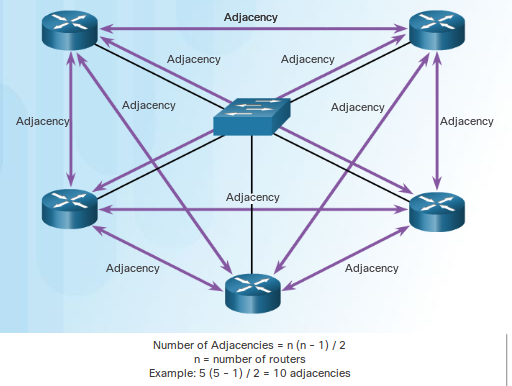
\includegraphics[width=0.7\textwidth]{multiple-adjacencies.png} 
\caption{Creating adjacencies with every neighbors in multiaccess network}
\label{multiple-adjacencies}
\end{figure}
	
\paragraph{Designated Router (DR)} is the solution to the problems on multiaccess network. On multiaccess networks and multiaccess networks only, OSPF elects a DR to be the collection and distribution point for LSPs sent and received. The router with the  The router ID of DR can be viewed using \texttt{show ip ospf interface} command on any routers within the multiaccess network.
	
\paragraph{Backup Designated Router (BDR)} is also elected. The BDR listens passively to this exchange and maintains a relationship with all the routers. If the DR stops producing Hello packets, the BDR promotes itself and assumes the role of DR.
	
\paragraph{DROTHER} All other routers become DROTHERs (a router that is neither the DR nor the BDR). Each DROTHER forms full adjacencies (Full state) with the DR and BDR and form 2-way adjacencies (Two-way state) with any DROTHERs (see figure \ref{DR-adjacency}). DROTHERs only send their LSPs to the DR and BDR using the multicast address 224.0.0.6 (all DR routers). All DROTHER routers still receive Hello packets from each other.
	
\begin{figure}[hbtp]
\centering
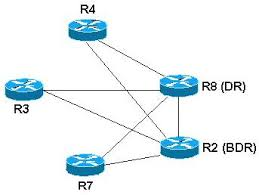
\includegraphics[width=0.4\textwidth]{pictures/dr-bdr.jpeg}
\caption{DROTHERs only form full adjacencies with the DR and BDR in the network}
\label{DR-adjacency}
\end{figure}

\subsection{Router ID}

Every router requires a router ID to participate in an OSPF domain. The router ID is used by the OSPF-enabled router to:

\begin{itemize}
\item Uniquely identify the router
\item Participate in DR election 
\end{itemize}

Cisco routers derive the router ID in one of three ways and with the following precedence: 

\begin{enumerate}
\item IP address configured with the OSPF router-id command, if present 
\item Highest IP address of any of the router’s loopback addresses, if present 
\item Highest active IP address on any of the router’s physical interfaces
\end{enumerate}

\subsection{Election decision}
	
The OSPF DR and BDR election decision is based on the following criteria, in sequential order:

\begin{enumerate}
\item The routers in the network elect the router with the highest interface priority as the DR. The router with the second highest interface priority is elected as the BDR.
\item If the interface priorities are equal, then the router with the highest router ID is elected the DR. The router with the second highest router ID is the BDR.
\end{enumerate}
	
After the DR is elected, it remains the DR until one of the following events occurs:

\begin{itemize}
\item The DR fails
\item The OSPF process on the DR fails or is stopped
\item The multiaccess interface on the DR fails or is shutdown
\end{itemize}
	
OSPF DR and BDR elections are not pre-emptive. If a new router with a higher priority or higher router ID is added to the network after the DR and BDR election, the newly added router does not take over the DR or the BDR role. This is because those roles have already been assigned. The addition of a new router does not initiate a new election process.\\

If the DR fails, the BDR is automatically promoted to DR. This is the case even if a new router A with a higher priority or router ID is added to the network after the initial DR/BDR election. However, after a BDR is promoted to DR, a new BDR election occurs and the router A is elected as the new BDR.

\section{OSPF area}
An OSPF area is a group of routers that share the same link-state information in their LSDBs. An instance of OSPF can have several areas (called Multi-area OSPF).

\subsection{Advantages of OSPF area}

\begin{itemize}
\item Smaller routing table (There are fewer routing table entries as network addresses can be summarized between areas.)
\item Reduced link-state update overhead (Fewer routers exchanging LSAs because LSA flooding stops at the area boundary.)
\item Reduced frequency of SPF calculations (Routing still occurs between the areas, however, the CPU intensive routing operation of recalculating the SPF algorithm is done only for routes within an area.)
\end{itemize}

\subsection{Two-layer area hierarchy}

To make OSPF more efficient and scalable, OSPF is implemented in a two-layer area hierarchy:

\begin{itemize}
\item \textbf{Backbone (Transit) area} -- A backbone area directly connected with all other areas. All traffic moving from one area to another area must traverse the backbone area. Generally, end users are not found within a backbone area. The backbone area is also called OSPF area 0.
\item \textbf{Regular (Non-backbone) area} -- Connects users and resources. By default, a regular area does not allow traffic from another area to use its links to reach other areas. All traffic from other areas must cross a transit area.
\end{itemize}
	
\subsection{Types of routers}

There are four different types of OSPF routers:

\begin{itemize}
\item Internal router (have all interfaces in the same area)
\item Backbone router (reside in backbone area)
\item Area border router or ABR (have interfaces attached to multiple areas)
\item Autonomous System Boundary Router or ASBR (have at least one interface attached to an external network)
\end{itemize}

\section{Configuration}

\subsection{Recommendations}

The optimal number of routers per area varies based on factors such as network stability, but Cisco recommends the following guidelines:
\begin{itemize}
\item An area should have no more than 50 routers.
\item A router should not be in more than three areas.
\item Any single router should not have more than 60 neighbors.
\end{itemize}

Also keep the following notes in mind:
\begin{itemize}
\item Propagating type 3 and 5 LSAs can cause significant flooding problems. For this reason, it is strongly recommended that manual route summarization be configured on the ABRs and ASBR.
\item For routers to become adjacent, their Hello interval, Dead interval, process ID and subnet masks must match.
\item  The dead interval must be larger than Hello interval.
\end{itemize}

\subsection{OSPF for IPv4}

\begin{enumerate}
\item Enable OSPF routing with process ID
	\begin{verbatim}
	R1(config)# router ospf 1
	\end{verbatim}
	
\item Configure the network statements for directly connected network
	\begin{verbatim}
	R1(config-router)# network 192.168.1.0 0.0.0.255 area 0 
	R1(config-router)# network 192.168.12.0 0.0.0.3 area 1 
	R1(config-router)# network 192.168.13.0 0.0.0.3 area 2
	\end{verbatim}
	
\item Configure passive interfaces
	\begin{verbatim} 
	R1(config-rtr)# passive-interface g0/0 
	R1(config-rtr)# passive-interface g0/1
	\end{verbatim}	

\item If there are too many passive interfaces, you can make all interfaces of the router to be passive using \verb|passive-interface default|, then configure necessary interface to be active again using \verb|no passive-interface|
	\begin{verbatim}
	R1(config-router)# passive-interface default
	R1(config-router)# no passive-interface s0/0/0
	R1(config-router)# no passive-interface s0/0/1
	\end{verbatim}		
	
\item Propagating a default static route. \note Do not use \verb|redistribute static| as this command will not recognize default static route (due to auto summarization, it only recognizes classful route).
	\begin{verbatim}
	R1(config)# router ospf 1
	R1(config-router)# default-information originate
	\end{verbatim}
	
\item Verify configuration using the following commands:
	\begin{itemize}
	\item \verb|show ip protocols|
	\item \verb|show ip ospf neighbor|
	\item \verb|show ip route ospf|
	\item \verb|show ip ospf|
	\item \verb|show ip ospf interface brief|
	\end{itemize}		
\end{enumerate}

\subsection{OSPF for IPv6}

\begin{enumerate}
\item Enable IPv6 routing on the router
	\begin{verbatim}
	R1(config)# ipv6 unicast-routing 
	\end{verbatim}
	
\item Enable OSPF for IPv6
	\begin{verbatim}
	R1(config)# ipv6 router ospf 1 
	R1(config-rtr)# no shutdown 
	\end{verbatim}	
	
\item Assign a router ID to each router
	\begin{verbatim}
	R1(config)# ipv6 router ospf 1 
	R1(config-rtr)# router-id 1.1.1.1
	\end{verbatim}

\item Configure passive interfaces
	\begin{verbatim}
	R1(config)# ipv6 router ospf 1 
	R1(config-rtr)# passive-interface g0/0 
	\end{verbatim}
	
\item If there are too many passive interfaces, you can make all interfaces of the router to be passive using \verb|passive-interface default|, then configure necessary interface to be active again using \verb|no passive-interface|
	\begin{verbatim}
	R1(config-router)# passive-interface default
	R1(config-router)# no passive-interface s0/0/0
	R1(config-router)# no passive-interface s0/0/1
	\end{verbatim}	
	
\item Configure OSPF for IPv6 with area number on each interface
	\begin{verbatim}
	R1(config)# interface g0/0 
	R1(config-if)# ipv6 ospf 1 area 0
	R1(config-if)# no shutdown
	R1(config-if)# interface g0/1       
	R1(config-if)# ipv6 ospf 1 area 55
	R1(config-if)# no shutdown
	\end{verbatim}     
	
\end{enumerate}	

\subsection{Summarization}

The following command enables Inter-area route summarization (for ABRs only). It summarizes all routes in an area to the specified summary address.

\begin{verbatim}
R1(config)# router ospf 1
R1(config-router)# area 1 range 192.168.64.0 255.255.224.0
\end{verbatim}

The following command enables External route summarization (for ASBRs only). It advertises a single route for all redistributed routes that are covered by a specified network.

\begin{verbatim}
R1(config)# router ospf 1
R1(config-router)# summary-address 192.168.64.0 255.255.224.0
\end{verbatim}

\subsection{Priority}

Configure OSPF priority for each interface. The higher the priority value (from 0 to 255), the more likely the router becomes the DR or BDR on the interface.	The priority of 0 means that the router will never  become a DR or BDR. On the other hand, 255 means the router will always be DR or BDR. As for IPv6, replace \verb|ip| by \verb|ipv6|.
	\begin{verbatim}
	R1(config)# interface g0/0 
	R1(config)# ip ospf priority 150
	\end{verbatim}
	
\subsection{Dead and Hello interval}

Configure OSPF Dead interval, Hello interval (in seconds). \note The Dead interval must not be smaller than the Hello interval. By default, the Dead interval is four times the Hello interval. As for IPv6, replace \verb|ip| by \verb|ipv6|.
	\begin{verbatim}
	R1(config)# interface g0/0
	R1(config-if)# ip ospf hello-interval 20 
	R1(config-if)# ip ospf dead-interval 80
	\end{verbatim}
	
\subsection{Reference bandwidth}	

Change reference bandwidth to 1000 Mb/s.
	\begin{verbatim}
	R1(config)# interface g0/0
	R1(config-if)# auto-cost reference-bandwidth 1000
	\end{verbatim}
	
\subsection{Assign OSPF cost}	

Directly assign OSPF cost. The cost is a number between 1 and 65,535. As for IPv6, replace \verb|ip| by \verb|ipv6|.
	\begin{verbatim}
	R1(config)# interface g0/0
	R1(config-if)# ip ospf cost 1564
	\end{verbatim}

\subsection{Verification}
As for IPv6, replace \verb|ip| by \verb|ipv6|.
\begin{enumerate} 
\item Examine the neighbor adjacencies using \verb|show ipv6 ospf neighbors|
\item Examine the IPv6 EIGRP routing table using \verb|show ipv6 route ospf|
\item Examine the EIGRP topology using \verb|show ipv6 ospf interface|
\item Verify the parameters and current state of the active IPv6 routing protocol processes using \verb|show ipv6 protocols|	
\end{enumerate}